What is the $\tan(\alpha\degree + \beta\degree)$

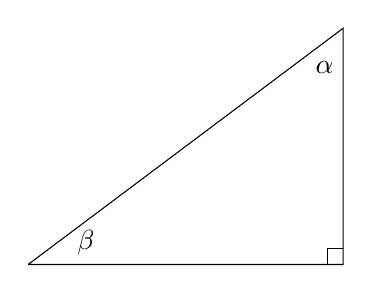
\begin{tikzpicture} 
\draw(0,0)--(4,0)--(4,3)--(0,0); 
\draw(3.8,0)--(3.8,0.2)--(4,0.2); 
\draw(4,2.7)node[anchor=north east]{$\alpha \degree$}; 
\draw(0.5,0)node[anchor=south west]{$\beta \degree$}; 
\end{tikzpicture} 

\ifsat
	\begin{enumerate}[label=\Alph*)]
		\item   $0$
		\item  $1$ 
		\item  $\sqrt{3}$ 
		\item  $undefined$ %
	\end{enumerate}
\else
\fi

\ifacteven
	\begin{enumerate}[label=\textbf{\Alph*.},itemsep=\fill,align=left]
		\setcounter{enumii}{5}
		\item   $0$
		\item  $1$ 
		\item  $\sqrt{3}$ 
		\addtocounter{enumii}{1}
		\item  $\frac{\sqrt{3}}{3}$ 
		\item  $undefined$ %
	\end{enumerate}
\else
\fi

\ifactodd
	\begin{enumerate}[label=\textbf{\Alph*.},itemsep=\fill,align=left]
		\item   $0$
		\item  $1$ 
		\item  $\sqrt{3}$ 
		\item  $\frac{\sqrt{3}}{3}$ 
		\item  $undefined$ %
	\end{enumerate}
\else
\fi

\ifgridin
  $undefined$ %

\else
\fi

